\documentclass[12pt]{article}

%\usepackage[utf8]{inputenc}
%\usepackage[T2B]{fontenc}
%\usepackage[english,russian]{babel}

%\frenchspacing

\usepackage{fullpage}
\usepackage{multicol,multirow}
\usepackage{tabularx}
\usepackage{ulem}
\usepackage[utf8]{inputenc}
\usepackage[russian]{babel}
\usepackage[table,xcdraw]{xcolor}
%\usepackage[open]{bookmark}
%\documentclass[xcolor=table]{beamer}
\usepackage{csquotes}
\usepackage{listings}
\usepackage{color}
\usepackage{tocloft}
\usepackage{amsmath}
\usepackage{empheq}
\usepackage{cancel}
\usepackage{cases}
\usepackage{wrapfig}
\usepackage{lipsum}
\usepackage{graphicx}
\usepackage{tikz}
\newcommand*\circled[1]{\tikz[baseline=(char.base)]{
  \node[shape=circle,draw,inner sep=1pt] (char) {#1};}}

%\usepackage{alltt}
%\usepackage{hyperref}
\lstset{
  literate={а}{{\selectfont\char224}}1
           {б}{{\selectfont\char225}}1
           {в}{{\selectfont\char226}}1
           {г}{{\selectfont\char227}}1
           {д}{{\selectfont\char228}}1
           {е}{{\selectfont\char229}}1
           {ё}{{\"e}}1
           {ж}{{\selectfont\char230}}1
           {з}{{\selectfont\char231}}1
           {и}{{\selectfont\char232}}1
           {й}{{\selectfont\char233}}1
           {к}{{\selectfont\char234}}1
           {л}{{\selectfont\char235}}1
           {м}{{\selectfont\char236}}1
           {н}{{\selectfont\char237}}1
           {о}{{\selectfont\char238}}1
           {п}{{\selectfont\char239}}1
           {р}{{\selectfont\char240}}1
           {с}{{\selectfont\char241}}1
           {т}{{\selectfont\char242}}1
           {у}{{\selectfont\char243}}1
           {ф}{{\selectfont\char244}}1
           {х}{{\selectfont\char245}}1
           {ц}{{\selectfont\char246}}1
           {ч}{{\selectfont\char247}}1
           {ш}{{\selectfont\char248}}1
           {щ}{{\selectfont\char249}}1
           {ъ}{{\selectfont\char250}}1
           {ы}{{\selectfont\char251}}1
           {ь}{{\selectfont\char252}}1
           {э}{{\selectfont\char253}}1
           {ю}{{\selectfont\char254}}1
           {я}{{\selectfont\char255}}1
           {А}{{\selectfont\char192}}1
           {Б}{{\selectfont\char193}}1
           {В}{{\selectfont\char194}}1
           {Г}{{\selectfont\char195}}1
           {Д}{{\selectfont\char196}}1
           {Е}{{\selectfont\char197}}1
           {Ё}{{\"E}}1
           {Ж}{{\selectfont\char198}}1
           {З}{{\selectfont\char199}}1
           {И}{{\selectfont\char200}}1
           {Й}{{\selectfont\char201}}1
           {К}{{\selectfont\char202}}1
           {Л}{{\selectfont\char203}}1
           {М}{{\selectfont\char204}}1
           {Н}{{\selectfont\char205}}1
           {О}{{\selectfont\char206}}1
           {П}{{\selectfont\char207}}1
           {Р}{{\selectfont\char208}}1
           {С}{{\selectfont\char209}}1
           {Т}{{\selectfont\char210}}1
           {У}{{\selectfont\char211}}1
           {Ф}{{\selectfont\char212}}1
           {Х}{{\selectfont\char213}}1
           {Ц}{{\selectfont\char214}}1
           {Ч}{{\selectfont\char215}}1
           {Ш}{{\selectfont\char216}}1
           {Щ}{{\selectfont\char217}}1
           {Ъ}{{\selectfont\char218}}1
           {Ы}{{\selectfont\char219}}1
           {Ь}{{\selectfont\char220}}1
           {Э}{{\selectfont\char221}}1
           {Ю}{{\selectfont\char222}}1
           {Я}{{\selectfont\char223}}1
}


\lstset{aboveskip=20pt,belowskip=20pt}

\definecolor{mygreen}{rgb}{0,0.6,0}
\definecolor{mygray}{rgb}{0.5,0.5,0.5}
\definecolor{mymauve}{rgb}{0.58,0,0.82}

\RequirePackage{listings}
\lstset{
  backgroundcolor=\color{white},   % choose the background color
  commentstyle=\color{mygreen},    % comment style
  escapeinside={\%*}{*)},          % if you want to add LaTeX within your code
  keywordstyle=\color{blue},       % keyword style
  stringstyle=\color{mymauve},     % string literal style
captionpos={bo},
numbers=left,
basicstyle=\ttfamily\footnotesize,
frame=lrtb,
breaklines=true,
tabsize=3,
language=C++,
%extendedchars=\true,
showtabs=false,
showspaces=false,
showstringspaces=false
}

\newcommand{\floor}[1]{\lfloor #1 \rfloor}
\newcommand{\CWPHeader}[1]{\addtocounter{section}{-1}\section{#1}}

% Заголовок курсовой работы
% Единственный аргумент --- ее тема
\newcommand{\CWHeader}[1]{\section*{#1}}

\setcounter{page}{1}
\thispagestyle{empty}

\begin{document}

\begin{center}
\bfseries

{\Large Московский авиационный институт\\ (национальный исследовательский университет)

}

\vspace{48pt}

{\large Факультет информационных технологий и прикладной математики
}

\vspace{36pt}


{\large Кафедра вычислительной математики и~программирования

}


\vspace{48pt}

Курсовой проект по курсу \enquote{Уравнения математической физики}

\end{center}

\vspace{72pt}

\begin{flushright}
\begin{tabular}{rl}
Студент: & Лихарев\ C.\,C. \\
Преподаватели: & Колесник\ С.\,А. \\ & Формалёв\ В.\,Ф. \\
Группа: & М8О-307Б \\
Дата: & \\
Оценка: & \\
Подпись: & \\
\end{tabular}
\end{flushright}

\vfill
\pagestyle{empty}
\begin{center}
\bfseries
Москва, \the\year
\end{center}

\newpage
\renewcommand{\cftdot}{}
\tableofcontents
\pagestyle{plain}
\setcounter{page}{1}
\newpage

\section{Задача №1}

\subsection{Формулировка задачи}

\indent

О распределении температур в конечном стержне $x \in [0; l]$ с начальным распределением $T_{0} = 300 (a^{2} = 10^{-6})$ и источником тепла $f(x, t) = 300 (1 + e^{-t})$, когда на левом конце задана температура $\mu_{1}=500$, а правый - теплоизолирован. Исследовать ортогональность и нормировку собственных функций, построить графики $u(x, t)$, $l=0,1$ м.

\subsection{Постановка задачи}

\begin{numcases}{}
u_{t} = a^{2}u_{xx} + 300(1 + e^{-t}), \qquad\quad \!\text{$x\in(0;l); t > 0$;}\\
u(x, 0) = \varphi (x) = 300k = T_{0}, \qquad \text{$x\in(0;l); t = 0$;}\\
\left.
\begin{split}
u(0, t) &= \mu_{1},\qquad\qquad\qquad\qquad\quad \!\!\!\text{$x = 0; t > 0$;}\\
u_{x}(l, t) &= 0,\qquad\qquad\qquad\qquad\quad \text{$x = l; t > 0$}\\
\end{split}
\,\,\,\,\,\right]
\end{numcases}

\subsection{Теоретические сведения}

\indent

Рассмотрим часть стержня на отрезке $[ x, x + \Delta x ]$ и воспользуемся законом сохранения количества тепла, согласно которому общее количество тепла на отрезке $[ x, x + \Delta x ]$ равно сумме полного количества тепла, прошедшему через границы, и полного количества тепла, образованного внутренними источниками. Формула общего количества тепла, которое необходимо сообщить участку стержня, чтобы повысить его температуру на $\Delta u$: $\Delta Q = C \rho S \Delta x \Delta u$, где $C$ -- удельная теплоёмкость материала, $S$ -- площадь поперечного сечения. Формула количества тепла прошедшего через левый конец участка стержня за время $\Delta t$: $Q_{1} = -kSu_{x}(x, t)\Delta t$, где $k$ -- коэффициент теплопроводности материала.

Аналогично, тепловой поток через правый конец участка вычисляется по формуле: $Q_{2} = -kSu_{x}(x+\Delta x, t)\Delta t$.

По закону сохранения тепла:

$$\Delta Q = Q_{1} - Q_{2} \Rightarrow C\rho S\Delta x \Delta u = kSu_{x}(x+\Delta x, t)\Delta t - kSu_{x}(x, t)\Delta t$$

Поделим на $S\Delta x \Delta t$ и устремим $\Delta x$ и $\Delta t$ к нулю, получим:

$$\frac{C\rho S\Delta x \Delta u}{S\Delta x \Delta t} = \frac{kSu_{x}(x+\Delta x, t)\Delta t - kSu_{x}(x, t)\Delta t}{S\Delta x \Delta t} \Rightarrow C\rho u_{t}=ku_{xx},$$

\noindent так как $\frac{\Delta u}{\Delta t} \rightarrow u_{t}$, $\frac{u_{x}(x+\Delta x, t) - u_{x}(x, t)}{\Delta x} \rightarrow u_{xx}$,

\noindent тогда уравнение теплопроводности имеет вид: $u_{t}=a^{2}u_{xx}$, где $a=\sqrt{\frac{k}{C\rho}}$ - коэффициент температуропроводимости.

Если внутри стержня имеются непрерывно распределённые источники тепла, уравнение становится неоднородным и обретает вид: $u_{t} = a^{2}u_{xx}+f(x,t)$, где $f(x, t)=\frac{1}{C\rho S}q(x, t)$. 

\subsection{Решение задачи}

\indent

Представим решение в виде суммы: $u(x, t) = v(x, t) + \mu_{1}$. Будем приводить начально-краевую задачу (1)-(3) к задаче с однородными граничными условиями (3).

Представим $u(x, t)$ в таком виде в уравнение (1), получим:

$$v_{t} =  a^{2}v_{xx} + 300(1 + e^{-t}), \eqno (4)$$

в начальное условие (2):

$$
\begin{cases}
u(x, 0) = \left.(v + \mu_{1})\right|_{t=0} = v(x, 0) + \mu_{1} = T_{0}; \\
v(x, 0) = T_{0} - \mu_{1}
\end{cases}
\eqno (5)
$$

и в граничные условия (3):

$$
\begin{cases}
u(0, t) = \left.(v + \mu_{1})\right|_{x=0} = v(0, t) + \mu_{1} = \mu_{1}; \\
u_{x}(l, t) = \left.(v + \mu_{1})_{x}\right|_{x=l} = v_{x}(l, t) = 0; \\
v(0, t) = 0; \\
v_{x}(l, t) = 0
\end{cases}
\eqno (6)
$$

Найдём собственные функции задачи (4)-(6), но с однородным волновым уравнением:

$$v_{t} = a^{2}v_{xx} \eqno (7)$$

Метод Фурье разделения переменных:

$$ v(x, t) = X(x) \cdot T(t) $$

Подставим в (7):

$$X(x) \cdot T'(t) = a^{2}X''(x) \cdot T(t)$$

$$\frac{T'(t)}{a^{2}T(t)} = \frac{X''(x)}{X(x)} = -\lambda^{2} = const$$

Получим две обыкновенные дифференциальные линейные уравнения:

$$T'(t) + a^{2}\lambda T(t) = 0,$$
$$X''(x) + \lambda X(x) = 0.$$

Подставляя $v(x, t)$ в виде $X(x) \cdot T(t)$ в граничные условия (6), получим:

$$u(0, t) = X(0) \cdot T(t) = 0;\,\,\,u_{x}(l, t) = X'(l) \cdot T(t) = 0$$

Поскольку равенства должны выполняться тождественно (зная, что $T(t) \neq 0$), то:

$$X(0) = 0;\,\,\,X'(l) = 0$$

Получим задачу Штурма-Лиувилля:

$$
\begin{cases}
X''(x) - \lambda^{2}X(x) = 0; \\
X(0) = 0; \\
X'(l) = 0
\end{cases}
$$

Рассмотрим различные значения $\lambda^{2}$:

\makeatletter
\@fleqntrue
\makeatother

\begin{equation*}
  \begin{split}
    1)\,\,\lambda^{2} > 0:
  \end{split}
\quad\quad
  \begin{split}
    \begin{cases}
      X(x) & = C_{1}e^{-\lambda x} + C_{2}e^{\lambda x}; \\
      X(0) & = C_{1} + C_{2} = 0; \\
      X'(l) & = -\lambda C_{1}e^{-\lambda l} + \lambda C_{2}e^{\lambda l} = 0
    \end{cases}
  \end{split}
\end{equation*}

\begin{multline*}
\begin{vmatrix}
     C_{1} & C_{2}\\ 
     -\lambda C_{1}e^{-\lambda l} & \lambda C_{2}e^{\lambda l}\\
\end{vmatrix}
\neq 0 \Rightarrow \text{единственное решение, а} \Rightarrow  \\
\Rightarrow C_{1} = C_{2} = 0\text{, что не удовлетворяет условиям задачи.} 
\end{multline*}


\begin{equation*}
  \begin{split}
    2)\,\,\lambda^{2} = 0:
  \end{split}
\quad\quad
  \begin{split}
    \begin{cases}
      X(x) & = C_{1}x + C_{2}; \\
      X(0) & = C_{2} = 0; \\
      X'(l) & = C_{1} = 0
    \end{cases}
  \end{split}
\quad\Rightarrow\quad
C_{1} = C_{2} = 0\text{, что снова не удовл. условиям задачи.}
\end{equation*}

\begin{equation*}
  \begin{split}
    3)\,\,\lambda^{2} < 0:
  \end{split}
\quad\quad
  \begin{split}
    \begin{cases}
      X(x) & = C_{1}\sin{\lambda x} + C_{2}\cos{\lambda x}; \\
      X(0) & = C_{2} = 0; \\
      X'(l) & = \lambda C_{1}\cos{\lambda l} = 0
    \end{cases}
  \end{split}
\quad\quad\quad
l=\frac{(1 + 2n)\pi}{2}, n=0,1,2\ldots
\end{equation*}

\makeatletter
\@fleqnfalse
\makeatother

\begin{equation*}
  \begin{split}
    \boxed{\lambda_{n} = \frac{(2n + 1)\pi}{2l}}
  \end{split}
\quad\quad
  \begin{split}
    \boxed{X_{n} = \sin{\lambda_{n}x} = \sin{\frac{(1 + 2n)\pi}{2l}x}}
  \end{split}
\quad\quad
\end{equation*}

Проверим ортогональность собственных функций:

$$ ( X_{n}(x), X_{k}(x) ) = \int\limits_0^l \sin \left( \frac{\pi(1 + 2n)}{2l}x \right) \cdot \sin \left( \frac{\pi(1 + 2k)}{2l}x \right)dx = $$

$$ = \frac{1}{2}\int\limits_0^l \left( \cos \left( \frac{\pi(1 + 2n)x}{2l} - \frac{\pi(1 + 2k)x}{2l} \right) - \cos \left( \frac{\pi(1 + 2n)x}{2l} + \frac{\pi(1 + 2k)x}{2l} \right) \right)dx = $$

$$ = \frac{1}{2}\int\limits_0^l \left( \cos \left( \frac{\pi(n - k)x}{l} \right) - \cos \left( \frac{\pi(n + k)x}{l} \right)\right)dx\,\, \circled{=}$$

Если $n\neq k$, то:

$$\circled{=} \,\,\,\frac{1}{2} \left( \left. \frac{l}{\pi (n - k)} \sin \left( \frac{\pi (n - k)x}{l} \right) \right|_0^l - \frac{l}{\pi (n + k)} \sin \left( \left. \frac{\pi (n + k) x}{l} \right) \right|_0^l \right)=$$

$$ = \frac{1}{2} \left( \frac{l}{\pi (n - k)} \sin{(\pi (n - k))} - \frac{l}{\pi (n + k)} \sin{(\pi (n + k))} \right) = 0;$$

Если $n=k$, то:

$$\circled{=} \,\,\,\frac{1}{2}\int\limits_0^l \left( 1 - \cos \left( \frac{\pi(n + k)x}{l} \right) \right)dx = \frac{1}{2} \left( \left. x \right|_0^l - \cancelto{0}{\left. \frac{l}{\pi (n + k)} \sin \left( \frac{\pi (n + k)x}{l} \right) \right|_0^l} \right) = \frac{l}{2} $$

Квадрат нормы собственных функций:

$$\|X_{n}\|^{2} = \int\limits_0^l X_{n}^{2}(x)dx = \int\limits_0^l \sin^{2}{\lambda_{n}x}dx = \int\limits_0^l \frac{1 - \cos{2\lambda_{n}x}}{2}dx = \frac{l}{2} - \left. \frac{1}{4} \sin{2\lambda_{n}x}\right|_0^l = \frac{l}{2} $$

Решение задачи (4)-(6) с неоднородным уравнением будем искать в виде ряда по собственным функциям однородной задачи:

$$v(x, t) = \sum_{n=0}^{\infty}T_{n}(t)X_{n}(x) = \sum_{n=0}^{\infty}T_{n}(t)\sin \left( \frac{\pi (1 + 2n)}{2l}x \right)$$

Подставим функцию $v(x, t)$ в таком виде в неоднородное уравнение (4) в начальное условие (5):

$$\sum_{n=0}^{\infty}T'_{n}(t)\cdot \sin \left( \frac{\pi (1 + 2n)}{2l}x \right) = a^{2}\sum_{n=0}^{\infty} \left( -\frac{\pi^{2}(1 + 2n)^{2}}{4l^{2}} \right) T_{n}(t)\cdot \sin \left( \frac{\pi(1 + 2n)}{2l}x \right) + 300(1 + e^{-t}),$$

$$v(x, 0) = \sum_{n=0}^{\infty}T_{n}(0) \cdot \sin \left( \frac{\pi (1 + 2n)}{2l}x \right) = T_{0} - \mu_{1}.$$

Разложим неоднородность $300(1+e^{-t})$ в ряд Фурье по собственным \linebreak функциям $\left\{ \sin \left( \frac{\pi (1 + 2n)}{2l}x \right)  \right\}_{n=0}^{\infty}$.

$$300(1 + e^{-t}) = 300(1 + e^{-t}) \cdot \sum_{n=0}^{\infty} f_{n} \cdot \sin \left( \frac{\pi (1 + 2n)}{2l}x \right)$$

Коэффициенты разложения равны:

$$f_{n} = \frac{(1, X_{n}(x))}{\|X_{n}\|^{2}} = \frac{2}{l} \int\limits_0^l \sin \left( \frac{\pi(1 + 2n)}{2l}x \right)dx = \frac{2}{l} \cdot \left( - \frac{2l}{\pi (1 + 2n)} \right) \cdot \left. \cos \left( \frac{\pi(1 + 2n)}{2l}x \right) \right|_0^l=$$

$$ = - \frac{4}{\pi(1 + 2n)} \cdot \left( \cos \left( \frac{\pi(1 + 2n)}{2} \right) - 1 \right) = \frac{4}{\pi(1 + 2n)}$$

Подставляем полученное разложение в уравнение и начальное условие:

\begin{multline*}
\sum_{n=0}^{\infty}T'_{n}(t)\cdot \sin \left( \frac{\pi(1 + 2n)}{2l}x \right) = a^{2}\sum_{n=0}^{\infty} \left( -\frac{\pi^{2}(1 + 2n)^{2}}{4l^{2}} \right) \cdot T_{n}(t) \cdot \sin \left( \frac{\pi(1 + 2n)}{2l}x \right) + \\
+ 300(1 + e^{-t}) \cdot \sum_{n=0}^{\infty} f_{n} \cdot \sin \left( \frac{\pi(1 + 2n)}{2l}x \right),
\end{multline*}

$$\sum_{n=0}^{\infty}T_{n}(0) \cdot \sin \left( \frac{\pi(1 + 2n)}{2l}x \right) = (T_{0} - \mu_{1}) \cdot \sum_{n=0}^{\infty} f_{n} \cdot \sin \left( \frac{\pi(1 + 2n)}{2l}x \right),$$

Учитывая полноту системы собственных функций $\left\{ \sin \left( \frac{\pi (1 + 2n)}{2l}x \right)  \right\}_{n=0}^{\infty}$ на отрезке $[0; l]$ и сравнивая коэффициенты при одинаковых функциях $\sin \left( \frac{\pi (1 + 2n)}{2l}x \right)$, получим следующие задачи Коши для функций $T_{n}(t) (n=0,1,2\ldots).$

$$
\begin{cases}
T'_{n}(t) = - \frac{a^{2}\pi^{2}(1 + 2n)^{2}}{4l^{2}}T_{n}(t) + 300f_{n}(1 + e^{-t});\\
T_{n}(0) = (T_{0} - \mu_{1}) \cdot f_{n}
\end{cases}
$$

Общее решение уравнения:

$$T_{n}(t) = A_{n}e^{- \frac{a^{2}\pi^{2}(1 + 2n)^{2}}{4l^{2}}t} + T_{n_{\text{част}}}(t)$$

Частное решение неоднородного уравнения $T_{n_{\text{част}}}(t)$ ищем исходя из вида неоднородности, т.е. в виде:  

$$T_{n_{\text{част}}}(t) = C_{n} + D_{n}e^{-t}$$

Подставляем в уравнение:

$$-D_{n}e^{-t} = -\frac{a^{2}\pi^{2}(1 + 2n)^{2}}{4l^{2}}\left( C_{n} + D_{n}e^{-t}\right) + 300 f_{n} (1 + e^{-t})$$

\begin{equation*}
\begin{aligned}
e^{-t}: \\
\\
1:
\end{aligned}
\quad \left\{
\begin{aligned}
       -D_{n} & = -\frac{a^{2}\pi^{2}(1 + 2n)^{2}}{4l^{2}} D_{n} + 300f_{n} \\
       0 & = -\frac{a^{2}\pi^{2}(1 + 2n)^{2}}{4l^{2}} C_{n} + 300f_{n}
\end{aligned}
\right.
\end{equation*} 

Отсюда:

\begin{equation*}
  \begin{split}
    C_{n} = \frac{1200l^{2}f_{n}}{a^{2}\pi^{2}(1 + 2n)^{2}};
  \end{split}
\quad\quad
  \begin{split}
    D_{n} = \frac{300f_{n}}{\frac{a^{2}\pi^{2}(1 + 2n)^{2}}{4l^{2}} - 1} = \frac{1200l^{2}f_{n}}{a^{2}\pi^{2}(1 + 2n)^{2} - 4l^{2}};
  \end{split}
\end{equation*}

$$T_{n_{\text{част}}}(t) = \frac{1200l^{2}f_{n}}{a^{2}\pi^{2}(1 + 2n)^{2}} + \frac{1200l^{2}f_{n}}{a^{2}\pi^{2}(1 + 2n)^{2}-4l^{2}} \cdot e^{-t}=$$

$$= 1200l^{2}f_{n} \left( \frac{1}{a^{2}\pi^{2}(1 + 2n)^{2}} + \frac{e^{-t}}{a^{2}\pi^{2}(1 + 2n)^{2} - 4l^{2}} \right)$$

$$T_{n}(t) = A_{n}e^{-\frac{a^{2}\pi^{2}(1 + 2n)^{2}}{4l^{2}}t} + 1200l^{2}f_{n} \left( \frac{1}{a^{2}\pi^{2}(1 + 2n)^{2}} + \frac{e^{-t}}{a^{2}\pi^{2}(1 + 2n)^{2} - 4l^{2}} \right)$$

Коэффициенты $A_{n}$ найдём из начального условия:

$$T_{n}(0) = A_{n} + 1200l^{2}f_{n}  \left( \frac{1}{a^{2}\pi^{2}(1 + 2n)^{2}} + \frac{1}{a^{2}\pi^{2}(1 + 2n)^{2} - 4l^{2}} \right) = (T_{0} - \mu_{1})f_{n}$$

$$A_{n} = (T_{0} - \mu_{1})f_{n} - 1200l^{2}f_{n} \left( \frac{1}{a^{2}\pi^{2}(1 + 2n)^{2}} + \frac{1}{a^{2}\pi^{2}(1 + 2n)^{2} - 4l^{2}} \right)$$

\begin{multline*}
T_{n}(t) =  \left( (T_{0} - \mu_{1})f_{n} - 1200l^{2}f_{n} \left( \frac{1}{a^{2}\pi^{2}(1 + 2n)^{2}} + \frac{1}{a^{2}\pi^{2}(1 + 2n)^{2} - 4l^{2}} \right) \right)e^{-\frac{a^{2}\pi^{2}(1 + 2n)^{2}}{4l^{2}}} + \\
+1200l^{2}f_{n}\left( \frac{1}{a^{2}\pi^{2}(1 + 2n)^{2}} + \frac{e^{-t}}{a^{2}\pi^{2}(1 + 2n)^{2} - 4l^{2}} \right) = 
\end{multline*}

$$ = (T_{0} - \mu_{1})f_{n}e^{-\frac{a^{2}\pi^{2}(1 + 2n)^{2}}{4l^{2}}t} + 1200l^{2}f_{n}\left( \frac{1}{a^{2}\pi^{2}(1 + 2n)^{2}} + \frac{e^{-t}}{a^{2}\pi^{2}(1 + 2n)^{2} - 4l^{2}} \right) \cdot (1 - e^{-\frac{a^{2}\pi^{2}(1 + 2n)^{2}}{4l^{2}}t}).$$

$\Rightarrow$ решение задачи (4)-(6) имеет вид:

\begin{multline*}
v(x, t) = \sum_{n=0}^{\infty}f_{n} \left( (T_{0} - \mu_{1})e^{-\frac{a^{2}\pi^{2}(1 + 2n)^{2}}{4l^{2}}t} + 1200l^{2} \left( \frac{1}{a^{2}\pi^{2}(1 + 2n)^{2}} + \frac{e^{-t}}{a^{2}\pi^{2}(1 + 2n)^{2} - 4l^{2}} \right) \cdot \right. \\ 
\left. \cdot \left( 1 - e^{-\frac{a^{2}\pi^{2}(1 + 2n)^{2}}{4l^{2}}t} \right) \right) \cdot \sin {\frac{\pi(1 + 2n)}{2l}x}
\end{multline*}

Решение задачи (1)-(3) будет:

$$u(x, t) = \mu_{1} + \sum_{n=0}^{\infty}f_{n} \left( (T_{0} - \mu_{1})e^{-\frac{a^{2}\pi^{2}(1 + 2n)^{2}}{4l^{2}}t} + 1200l^{2} \left( \frac{1}{a^{2}\pi^{2}(1 + 2n)^{2}} + \frac{e^{-t}}{a^{2}\pi^{2}(1 + 2n)^{2} - 4l^{2}} \right) \cdot \right.$$

$$\left. \cdot \left( 1 - e^{-\frac{a^{2}\pi^{2}(1 + 2n)^{2}}{4l^{2}}t} \right) \right) \cdot \sin \left( {\frac{\pi(1 + 2n)}{2l}x} \right) = \mu_{1} + \sum_{n=0}^{\infty} \frac{4}{\pi(1 + 2n)} \left( (T_{0} - \mu_{1})e^{-\frac{a^{2}\pi^{2}(1 + 2n)^{2}}{4l^{2}}t} + \right. $$

$$ \left. + 1200l^{2} \left( \frac{1}{a^{2}\pi^{2}(1 + 2n)^{2}} + \frac{e^{-t}}{a^{2}\pi^{2}(1 + 2n)^{2} - 4l^{2}} \right) \cdot \left( 1 - e^{-\frac{a^{2}\pi^{2}(1 + 2n)^{2}}{4l^{2}}t} \right) \right) \cdot \sin \left( {\frac{\pi(1 + 2n)}{2l}x} \right)$$

Подставим $l = 0,1 \text{м}; a^{2} = 10^{-6}; \mu_{1} = 500; T_{0} = 300$:

\begin{multline*}
u(x, t) = 500 + \sum_{n=0}^{\infty} \frac{4}{\pi(1 + 2n)} \left( -200e^{\frac{-\pi^{2}(1 + 2n)^{2}}{4 \cdot 10^{4}}t} + 12 \left( \frac{10^{6}}{\pi^{2}(1 + 2n)^{2}} + \frac{10^{6}e^{-t}}{\pi^{2}(1 + 2n)^{2} - 4 \cdot 10^{4}} \right) \cdot \right. \\
\left. \cdot \left( 1 - e^{-\frac{\pi^{2}(1 + 2n)^{2}}{4 \cdot 10^{4}}t} \right)\right) \sin{(5\pi(1 + 2n)x)} \end{multline*}

\pagebreak

Построим графики функции $u(x, t)$ в разные моменты времени:

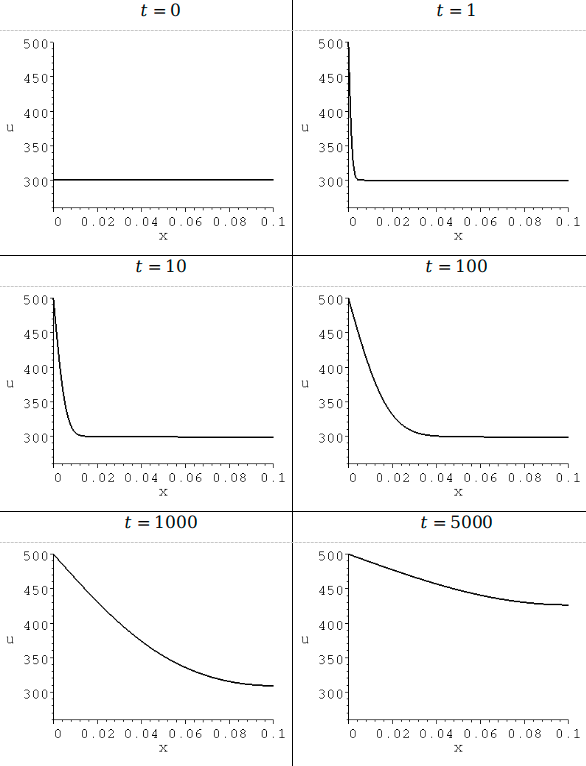
\includegraphics[width=0.8\linewidth]{task1.png}

По этой картине можно сказать следующее, при $t = 0$ значение $u$ будет равным 300, что верно, благодаря условию $u(x, 0) = \varphi(x)$. При изменении $t$ мы видим, что график функции $u(x, t)$ принимает своё начало в 500, что тоже верно, благодаря другому условию: $u(0, t) = \mu_{1}(t)$. При небольших $t$ можно чётко увидеть, как функция $u$ к концу стержня стремится к 300, что соответствует условию $u_{x}(l, t) = 0$. В целом график функции полностью соответствует краевым условиям задачи.

\pagebreak
\section{Задача №2}

\subsection{Формулировка задачи}

\indent

О вынужденных колебаниях конечного стержня $x \in [0; l], l = 0,1 \text{м}, a^{2} = 10^{6}, f(x, t) = x + t$ с нулевым начальным отклонением и начальной скоростью, когда левый конец зажат, а правый свободен. Результат $u(x, t)$ оформить графически.

\subsection{Постановка задачи}

\setcounter{equation}{0}

\begin{numcases}{}
u_{tt} = a^{2}u_{xx} + f(x, t), \qquad\qquad\qquad\qquad\qquad \,\,\text{$0 < x < l, t > 0$;}\\
\left.
\begin{split}
u(x, 0) = 0, \qquad\qquad\qquad\qquad\qquad\qquad\qquad \text{$0 < x < l, t = 0$;}\\
u_{t}(x, 0) = 0, \qquad\qquad\qquad\qquad\qquad\qquad\qquad \text{$0 < x < l, t = 0$;}\\
\end{split}
\,\,\,\,\,\right]
\\
\left.
\begin{split}
u(0, t) &= 0, \qquad\qquad\qquad\qquad\qquad\qquad\qquad \,\text{$x = 0, t > 0$;}\\
u_{x}(l, t) &= 0, \qquad\qquad\qquad\qquad\qquad\qquad\qquad\, \text{$x = l, t > 0$}
\end{split}
\,\,\,\,\,\right]
\end{numcases}

\subsection{Теоретические сведения}

\indent

Уравнения с частными производными 2-го порядка гиперболического типа наиболее часто встречаются в физических задачах, связанных с процессами колебаний. Простейшее уравнение гиперболического типа:

$$u_{xx} - u_{yy} = 0$$

\noindent обычно называют уравнением колебаний струны.

Уравнения продольных колебаний для струны, стержня и пружины записываются одинаково. Рассмотрим стержень, расположенный на отрезке $(0, l)$ оси $x$. Процесс продольных колебаний может быть описан одной функцией $u(x, t)$, представляющей в момент $t$ смещение точки, имевшей в положении равновесия абсциссу $x$. При продольных колебаниях это смещение происходит вдоль стержня. При выводе уравнения будем предполагать, что натяжения, возникающие в процессе колебания, следуют закону Гука.

Подсчитаем относительное удлинение элемента $(x, x + \Delta x)$ в момент $t$. Координаты концов этого элемента в момент $t$ имеют значения $x + u(x, t), x + \Delta x + u(x + \Delta x, t)$, а относительное удлинение равно:

$$\frac{\left( \Delta x + u(x + \Delta x, t) - u(x, t)\right) - \Delta x}{\Delta x} = u_{x}(x + \theta \Delta x, t) \quad\quad 0 \le \theta \le 1$$ 

Переходя к пределу при $\Delta x \rightarrow 0$, получим, что относительное удлинение в точке $x$ определяется функцией $u_{x}(x, t)$. В силу закона Гука натяжение $T(x, t)$ равно

$$T(x, t) = k(x)u_{x}(x, t),$$

\noindent где $k(x) - $ модуль Юнга в точке $x(k(x)) > 0$.

Пользуясь теоремой об изменении количества движения, получаем интегральное уравнение колебаний:

$$\int\limits_{x_{1}}^{x_{2}}\left( u_{t}(\xi, t_{2}) - u_{t}(\xi, t_{1})\right) \cdot \rho(\xi)d\xi = \int\limits_{t_{1}}^{t_{2}}\left( k(x_{2})u_{x}(x_{2}, \tau) - k(x_{1})u_{x}(x_{1}, \tau)\right)d\tau + \int\limits_{x_{1}}^{x_{2}} \int\limits_{t_{1}}^{t_{2}}F(\xi, \tau)d\xi d\tau,$$

\noindent где $F(x, t) -$ плотность внешней силы, рассчитанная на единицу длины.

Предположим существование и непрерывность вторых производных функции $u(x, t)$. Применяя теорему о среднем и совершая предельный переход при $\Delta x = x_{2} - x_{1} \rightarrow 0$ и $\Delta t = t_{2} - t_{1} \rightarrow 0$, приходим к дифференциальному уравнению продольных колебаний стержня:

$$[k(x)u_{x}]_{x} = \rho u_{tt} - F(x, t).$$

Если стержень однороден $(k(x) = const, \rho = const)$, то это уравнение записывают следующим образом:

\begin{equation*}
  \begin{split}
    u_{tt} = a^{2}u_{xx} + f(x, t)
  \end{split}
\quad\quad
  \begin{split}
    \left( a = \sqrt{\frac{k}{\rho}} \right),
  \end{split}
\quad\quad
  \begin{split}
    \text{где}\,\,\, f(x, t) = \frac{F(x, t)}{\rho}
  \end{split}
\quad\quad
\end{equation*}

\subsection{Решение задачи}

\indent

Найдём собственные функции задачи с однородным волновым уравнением:

$$u_{tt} = a^{2}u_{xx},\,\,\, 0 < x < l,\,\,\,t > 0 \eqno (4)$$

Метод Фурье разделения переменных: $u(x, t) = X(x)\cdot T(t)$.

Подставим в (4): $X(x) \cdot T''(t) = a^{2}X''(x) \cdot T(t)$

$$\frac{T''(t)}{a^{2}T(t)} = \frac{X''(x)}{X(x)} = -\lambda^{2} =const$$

\begin{equation*}
  \begin{split}
    T''(t) + a^{2}\lambda^{2}T(t) = 0
  \end{split}
\quad\quad
  \begin{split}
    X''(x) + \lambda^{2}X(x) = 0
  \end{split}
\quad\quad
\end{equation*}

Подставим $u(x, t)$ в виде $X(x)\cdot T(t)$ в граничные условия (3):

$$u(0, t) = X(0)\cdot T(t) = 0, \,\,\, u_{x}(l, t) = X'(l)\cdot T(t) = 0$$

\begin{equation*}
  \begin{split}
    \text{Задача Штурма-Лиувилля:}
  \end{split}
\quad\quad
  \begin{split}
  	\begin{cases}
  		X''(x) + \lambda^{2}X(x) = 0; \\
  		X(0) = 0; \\
  		X'(l) = 0
  	\end{cases}
  \end{split}
\quad\quad
  \begin{split}
    \frac{X''}{X} = -\lambda^{2}
  \end{split}
\quad\quad
\end{equation*}

\begin{equation*}
  \begin{split}
    \text{При}\,\,\, \lambda^{2} < 0:
  \end{split}
\quad\quad
  \begin{split}
  	\begin{cases}
  		X = C_{1}\sin{\lambda x} + C_{2}\cos{\lambda x};\\
  		X(0) = C_{2} = 0;\\
  		X'(l) = \lambda C_{1}\cos{\lambda l} = 0
  	\end{cases}
  \end{split}
\quad\quad
\end{equation*}

\begin{equation*}
  \begin{split}
    \lambda l = \frac{(1 + 2n)\pi}{2},
  \end{split}
\quad\quad
  \begin{split}
    n=0,1,2\ldots
  \end{split}
\quad\quad
\end{equation*}

\begin{equation*}
  \begin{split}
    \boxed{\lambda_{n} = \frac{(1 + 2n)\pi}{2l}}
  \end{split}
\quad\quad
  \begin{split}
    \boxed{X_{n} = \sin{\frac{(1 + 2n)\pi}{2l}x}}
  \end{split}
\quad\quad
\end{equation*}

Разложим в ряд по собственным функциям искомую $u(x, t)$:

$$u(x, t) = \sum_{n=0}^{\infty}T_{n}(t)X_{n}(x) = \sum_{n=0}^{\infty} T_{n}(t) \sin \left( \frac{\pi(1 +2n)}{2l}x \right)$$

Подставим $u(x, t)$ в (1) и начальные условия (2):

$$\sum_{n=0}^{\infty}T''_{n}(t)\cdot \sin \left( \frac{\pi(1 + 2n)}{2l}x \right) = a^{2}\sum_{n=0}^{\infty}\left( -\frac{\pi^{2}(1 + 2n)^{2}}{4l^{2}}\right) \cdot T_{n}(t) \cdot \sin\left( \frac{\pi(1 + 2n)}{2l}x \right) +x + t;$$

$$u(x, 0) = \sum_{n=0}^{\infty} T_{n}(0) \cdot \sin\left( \frac{\pi(1 + 2n)}{2l}x \right) = 0;$$

$$u_{t}(x, 0) = \sum_{n=0}^{\infty} T'_{n}(0) \cdot \sin\left( \frac{\pi(1 + 2n)}{2l}x \right) = 0$$

Также разложим неоднородность $x + t$ в ряд Фурье по собственным функциям $\left\{ \sin \left( \frac{\pi (1 + 2n)}{2l}x \right)  \right\}_{n=0}^{\infty}$:

$$ x + t = \sum_{n=0}^{\infty} f_{n} \cdot \sin \left( \frac{\pi(1 + 2n)}{2l}x \right) + t \cdot \sum_{n=0}^{\infty} g_{n} \cdot \sin \left( \frac{\pi(1 + 2n)}{2l}x \right).$$

Коэффициенты разложения равны:

$$\boldsymbol{f_{n}} = \frac{2}{l} \int\limits_0^l x \cdot \sin \left( \frac{\pi(1 + 2n)}{2l}x \right) dx = \frac{2}{l} \int\limits_0^l x \left( -\frac{2l}{\pi(1 + 2n)} \right)d \cos\left( \frac{\pi(1 + 2n)}{2l}x \right) = $$

$$= -\frac{4}{\pi(1 + 2n)} \cdot \left( \left. x \cdot \cos\left( \frac{\pi(1 + 2n)}{2l}x \right) \right|_{0}^{l} - \int\limits_0^l \cos \left( \frac{\pi(1 + 2n)}{2l}x \right) dx \right) = $$

$$ = -\frac{4}{\pi(1 + 2n)} \cdot \left( l\cdot \cos \left( \frac{\pi(1 + 2n)}{2}x \right) - \left. \frac{2l}{\pi(1 + 2n)} \cdot \sin \left( \frac{\pi(1 + 2n)}{2l}x \right) \right|_{0}^{l} \right) = $$

$$ = \frac{8l}{\pi^{2}(1 + 2n)^{2}} \cdot \sin \left( \frac{\pi(1 + 2n)}{2} \right) = \frac{8l(-1)^{n}}{\pi^{2}(1 + 2n)^{2}} $$

$$\boldsymbol{g_{n}} = \frac{2}{l} \int\limits_0^l \sin\left( \frac{\pi(1 + 2n)}{2l}x \right) dx = \frac{2}{l} \cdot \left. \left( -\frac{2l}{\pi(1 + 2n)} \right) \cdot \cos \left( \frac{\pi(1 + 2n)}{2l}x \right) \right|_{0}^{l} = $$

$$= - \frac{4}{\pi(1 + 2n)} \cdot \left( \cos \left( \frac{\pi(1 + 2n)}{2} \right) - 1 \right) = \frac{4}{\pi(1 + 2n)};$$

Подставляем полученное разложение в уравнение:

\begin{multline*}
\sum_{n=0}^{\infty} T''_{n}(t) \cdot \sin \left( \frac{\pi(1 + 2n)}{2l}x \right) = -\sum_{n=0}^{\infty} \frac{a^{2}\pi^{2}(1 + 2n)^{2}}{4l^{2}}T_{n}(t) \cdot \sin \left( \frac{\pi(1 + 2n)}{2l}x \right) +\\
+ \sum_{n=0}^{\infty} f_{n} \cdot \sin \left( \frac{\pi(1 + 2n)}{2l}x \right) + t \sum_{n=0}^{\infty} g_{n} \sin \left( \frac{\pi(1 + 2n)}{2l}x \right).
\end{multline*}

Учитывая полноту системы собственных функций $\left\{ \sin \left( \frac{\pi (1 + 2n)}{2l}x \right)  \right\}_{n=0}^{\infty}$ на отрезке $[0; l]$ и сравнивая коэффициенты при одинаковых функциях $\sin \left( \frac{\pi (1 + 2n)}{2l}x \right)$, получим следующие задачи Коши для функций $T_{n}(t)(n=0,1,2\ldots)$.

$$
\begin{cases}
T''_{n}(t) = - \frac{a^{2}\pi^{2}(1 + 2n)^{2}}{4l^{2}}T_{n}(t) + f_{n} + g_{n}t; \\
T_{n}(0) = 0, \quad\quad T'_{n}(0) = 0
\end{cases}
$$

Общее решение уравнения:

$$T_{n}(t) = A_{n} \cdot \cos \left( \frac{a\pi (1 + 2n)}{2l}t \right) + B_{n} \cdot \sin \left( \frac{a\pi (1 + 2n)}{2l}t \right) + T_{n_{\text{част}}}(t)$$

Частное решение неоднородного уравнения $T_{n_{\text{част}}}(t)$ ищем исходя из вида неоднородности, т.е. в виде:

$$T_{n_{\text{част}}}(t) = C_{n}t + D_{n}$$

Подставляем в уравнение $0 = - \frac{a^{2}\pi^{2}(1 + 2n)^{2}}{4l^{2}} (C_{n}t + D_{n}) + f_{n} + g_{n}t$

\begin{equation*}
\begin{aligned}
t: \\
\\
1:
\end{aligned}
\quad \left\{
\begin{aligned}
       0 & = -\frac{a^{2}\pi^{2}(1 + 2n)^{2}}{4l^{2}} C_{n} + g_{n}; \\
       0 & = -\frac{a^{2}\pi^{2}(1 + 2n)^{2}}{4l^{2}} D_{n} + f_{n}
\end{aligned}
\right.
\end{equation*}

Отсюда:

\begin{equation*}
  \begin{split}
    C_{n} = \frac{4l^{2}g_{n}}{a^{2}\pi^{2}(1 + 2n)^{2}};
  \end{split}
\quad\quad
  \begin{split}
    D_{n} = \frac{4l^{2}f_{n}}{a^{2}\pi^{2}(1 + 2n)^{2}};
  \end{split}
\end{equation*}

$$T_{n_{\text{част}}}(t) = \frac{4l^{2}g_{n}}{a^{2}\pi^{2}(1 + 2n)^{2}}t + \frac{4l^{2}f_{n}}{a^{2}\pi^{2}(1 + 2n)^{2}} = \frac{4l^{2}(f_{n} + g_{n}t)}{a^{2}\pi^{2}(1 + 2n)^{2}} $$

$$T_{n}(t) = A_{n}\cdot \cos\left( \frac{a\pi(1 + 2n)}{2l}t \right) + B_{n} \sin \left( \frac{a\pi(1 + 2n)}{2l}t \right) + \frac{4l^{2}(f_{n} + g_{n}t)}{a^{2}\pi^{2}(1 + 2n)^{2}}$$

$$T'_{n}(t) = \frac{a\pi(1 + 2n)}{2l} \left( -A_{n}\sin\left( \frac{a\pi(1 + 2n)}{2l}t \right) + B_{n} \cos \left( \frac{a\pi(1 + 2n)}{2l}t \right) \right) + \frac{4l^{2}g_{n}}{a^{2}\pi^{2}(1 + 2n)^{2}}$$

Коэффициенты $A_{n}, B_{n}$ найдём из начальных условий:

\begin{equation*}
  \begin{split}
    \begin{cases}
      T_{n}(0) = A_{n} + \frac{4l^{2}f_{n}}{a^{2}\pi^{2}(1 + 2n)^{2}} = 0;\\
      T'_{n}(0) = \frac{a\pi(1 + 2n)}{2l}B_{n} + \frac{4l^{2}g_{n}}{a^{2}\pi^{2}(1 + 2n)^{2}} = 0
    \end{cases}
  \end{split}
\Rightarrow
  \begin{split}
    \begin{cases}
      A_{n} = - \frac{4l^{2}f_{n}}{a^{2}\pi^{2}(1 + 2n)^{2}};\\
      B_{n} = - \frac{8l^{3}g_{n}}{a^{3}\pi^{3}(1 + 2n)^{3}}
    \end{cases}
  \end{split}
\end{equation*}

$$T_{n}(t) = - \frac{4l^{2}f_{n}}{a^{2}\pi^{2}(1 + 2n)^{2}} \cos \left( \frac{a\pi(1 + 2n)}{2l}t \right) - \frac{8l^{3}g_{n}}{a^{3}\pi^{3}(1 + 2n)^{3}} \sin \left( \frac{a\pi(1 + 2n)}{2l}t \right) + \frac{4l^{2}(f_{n} + g_{n}t)}{a^{2}\pi^{2}(1 + 2n)^{2}} =$$

$$ = \frac{8l^{3}}{a^{3}\pi^{3}(1 + 2n)^{3}} \left( \frac{a\pi(1 + 2n)}{2l}f_{n} \left( 1 - \cos \left( \frac{a\pi(1 + 2n)}{2l}t \right) \right) + g_{n} \left( \frac{a\pi(1 + 2n)}{2l}t - \sin \left( \frac{a\pi(1 + 2n)}{2l}t \right) \right) \right).$$

$\Rightarrow$ решение задачи (1) - (3) имеет вид:

\begin{multline*}
u(x, t) = \sum_{n=0}^{\infty} \frac{8l^{3}}{a^{3}\pi^{3}(1 + 2n)^{3}} \left( \frac{a\pi(1 + 2n)}{2l}f_{n} \left( 1 - \cos \left( \frac{a\pi(1 + 2n)}{2l}t \right) \right) + \right.\\
\left. + g_{n} \left( \frac{a\pi(1 + 2n)}{2l}t - \sin \left( \frac{a\pi(1 + 2n)}{2l}t \right) \right) \right) \sin \left( \frac{\pi(1 + 2n)}{2l}x \right) =
\end{multline*}

\begin{multline*}
= \sum_{n=0}^{\infty} \frac{8l^{3}}{a^{3}\pi^{3}(1 + 2n)^{3}} \left( \frac{a\pi(1 + 2n)}{2l} \cdot \frac{8l(-1)^{n}}{\pi^{2}(1 + 2n)^{2}} \left( 1 - \cos \left( \frac{a\pi(1 + 2n)}{2l}t \right) \right) + \right. \\
\left. + \frac{4}{\pi(1 + 2n)} \left( \frac{a\pi(1 + 2n)}{2l}t - \sin \left( \frac{a\pi(1 + 2n)}{2l}t \right) \right) \right) \sin \left( \frac{\pi(1 + 2n)}{2l}x \right) =
\end{multline*}

\begin{multline*}
= \frac{32l^{3}}{a^{3}\pi^{4}} \sum_{n=0}^{\infty} \frac{1}{(1 + 2n)^{4}} \left( a(-1)^{n} \left( 1 - \cos \left( \frac{a\pi(1 + 2n)}{2l}t \right) \right) - \right.\\
\left. - \sin \left( \frac{a\pi(1 + 2n)}{2l}t \right) + \frac{a\pi(1 + 2n)}{2l}t \right) \sin \left( \frac{\pi(1 + 2n)}{2l}x \right).
\end{multline*}

Подставим параметры задачи $l = 0,1 \text{м}, a^{2} = 10^{6}$:

\begin{multline*}
u(x, t) = \frac{32}{10^{6}\pi^{4}} \sum_{n=0}^{\infty} \frac{1}{(1 + 2n)^{4}} \left( 10^{3}(-1)^{n} \left( 1 - \cos \left( \frac{10^{3}\pi(1 + 2n)}{0.2}t \right) \right) - \right.\\
\left. - \sin \left( \frac{10^{3}\pi(1 + 2n)}{0.2}t \right) + \frac{10^{3}\pi(1 + 2n)}{0.2}t \right) \sin \left( \frac{\pi(1 + 2n)}{0.2}x \right) =
\end{multline*}

\begin{multline*}
= \frac{32}{10^{6}\pi^{4}} \sum_{n=0}^{\infty} \frac{1}{(1 + 2n)^{4}} \left( 1000(-1)^{n} \left( 1 - \cos (5000 \pi(1 + 2n)t) \right) - \right.\\
\left. - \sin \left(5000\pi(1 + 2n)t \right) + 5000\pi(1 + 2n)t \right) \sin \left( 5\pi(1 + 2n)x \right).
\end{multline*}

$\linebreak$
$\linebreak$

Построим графики функции $u(x, t)$ в разные моменты времени:

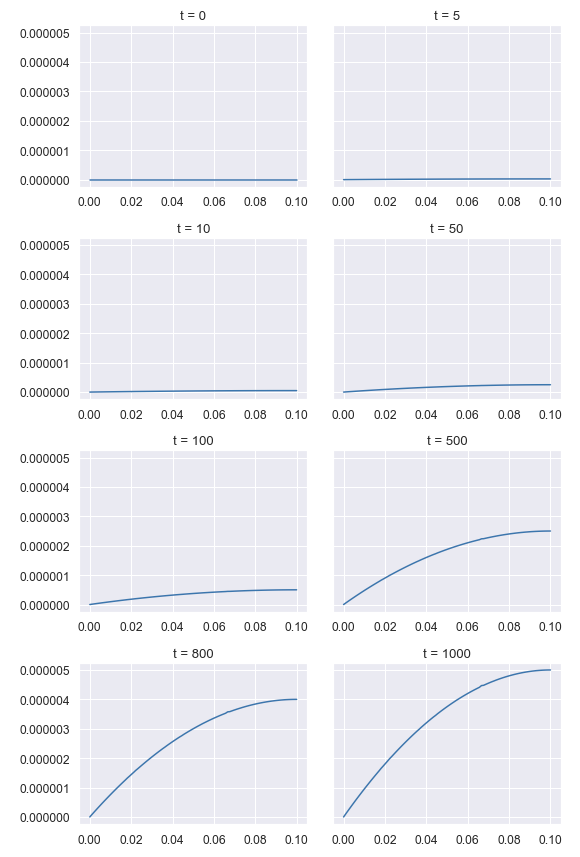
\includegraphics[width=0.8\linewidth]{task2.png}

Как мы видим, задан стержень и на его левом конце в разные моменты времени функция $u$ принимает значение 0. Это верно, поскольку по условию задачи, левый конец стержня зажат. При этом мы видим, что на правом конце функция меняется при изменении времени $t$, что тоже верно, так как правый конец свободен.

\pagebreak
\section{Задача №3}

\subsection{Формулировка задачи}

\indent

Решить задачу Дирихле для уравнения Лапласа в прямоугольнике $l_{1}\times l_{2}$, когда на верхней границе задан поток $\frac{\partial u(x, l_{2})}{\partial y} = \sin \left( \frac{\pi x}{l_{1}} \right)$, а на остальных границах заданы нулевые значения функции.

\subsection{Постановка задачи}

\begin{wrapfigure}{r}{0.25\textwidth}
    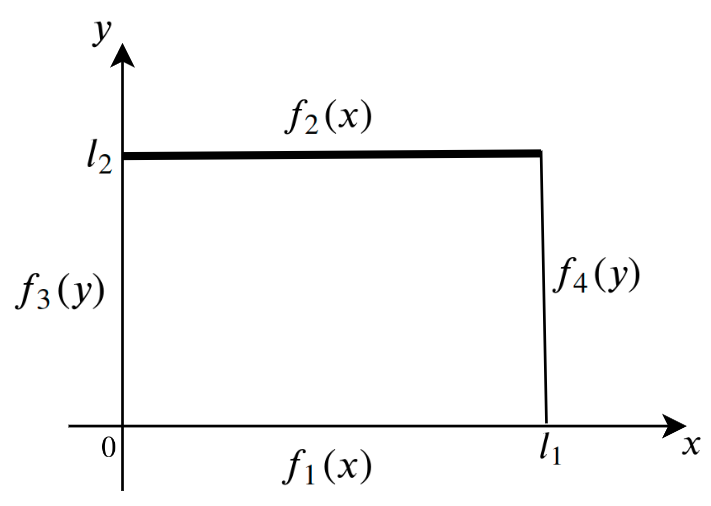
\includegraphics[width=0.34\textwidth]{task3_source.png}
\end{wrapfigure}
\leavevmode

\setcounter{equation}{0}

\begin{numcases}{}
\Delta u = 0\,\,\,\text{- условие Лапласа}, &\text{$0 < x < l_{1}; 0 < y < l_{2};$}\\
u(x, 0) = f_{1}(x) = 0;\\
u_{y}(x, l_{2}) = f_{2}(x) = \sin \left( \frac{\pi x}{l_{1}} \right);\\
u(0, y) = f_{3}(y) = 0;\\
u(l_{1}, y) = f_{4}(y) = 0
\end{numcases}
$\linebreak\linebreak\linebreak$

\subsection{Теоретические сведения}

\indent

При решении первой краевой задачи для прямоугольника требуется найти функцию $u$, удовлетворяющую уравнению (1) и граничным условиям (2)-(5) на границах прямоугольника.

Решим задачу методом разделения переменных, найдя частное решение уравнения (1) вида $u(x, y) = X(x)\cdot Y(y) \not\equiv 0$.

Подставляя это решение в оператор Лапласа: $X''Y + Y''X = 0$, получим:

$$\frac{X''}{X} = - \frac{Y''}{Y} = - \lambda^{2}\,\,\, \text{(задача Штурма-Лиувилля), где}\,\,\, \lambda = const.$$

Для нахождения функции $X$ получим уравнение второго порядка: $\frac{X''}{X} = -\lambda^{2}$, чтобы функция $u$ удовлетворяла нужному из условий, функция $X$ должна удовлетворять условиям: $X(a) = X(0) = 0$.

Далее задача решается совершенно обычным способом, а её общее решение этой задачи - функцию $u(x, y)$ можем искать в виде суммы основных решений.

\pagebreak

\subsection{Решение задачи}

\indent

Решим задачу методом разделения переменных: $u(x, y) = X(x) \cdot Y(y)$. Подставим в оператор Лапласа: $X''Y + Y''X = 0$

$$\frac{X''}{X} = -\frac{Y''}{Y} = -\lambda^{2}$$

В решении уравнения теплопроводности при $\lambda^{2} \geq 0$ решений нет.

\begin{equation*}
\begin{aligned}
\text{Рассмотрим}\,\,\, \lambda^{2} < 0: \\
\end{aligned}
\quad \left\{
\begin{aligned}
       & X'' + \lambda^{2}X = 0; \\
       & X = C_{1} \sin{\lambda x} + C_{2} \cos{\lambda x}
\end{aligned}
\right.
\end{equation*}  

Из граничных условий (4), (5) получим:

\begin{equation*}
  \begin{split}
    X(0) & = C_{2} = 0;\\
    X(l_{1}) & = C_{1} \sin{\lambda l_{1}} = 0;
  \end{split}
\quad\rightarrow\quad
  \begin{split}
    & \sin{\lambda l_{1}} = 0;\\
    & \lambda l_{1} = \pi n, \quad n=1,2,3\ldots
  \end{split}
\end{equation*}

\begin{equation*}
  \begin{split}
    \boxed{\lambda_{n} = \frac{\pi n}{l_{1}}}
  \end{split}
\quad\quad
  \begin{split}
    \boxed{X_{n}(x) = \sin{\frac{\pi n}{l_{1}}x}}
  \end{split}
\quad\quad
\end{equation*}

Найдём $Y(y)$:

\begin{equation*}
  \begin{split}
    - \frac{Y''}{Y} = \lambda^{2}
  \end{split}
\Rightarrow
  \begin{split}
  	& Y'' - \lambda^{2}Y = 0;\\
  	& Y = A_{n} \cdot e^{-\frac{\pi n}{l_{1}}y} + B_{n} \cdot e^{\frac{\pi n}{l_{1}}y}
  \end{split}
\end{equation*}

$$u(x, y) = \sum_{n=1}^{\infty} \sin{\frac{\pi n}{l_{1}}x}\cdot \left( A_{n}\cdot e^{-\frac{\pi n}{l_{1}}y} + B_{n} \cdot e^{\frac{\pi n}{l_{1}}y} \right)$$

Подставим в краевые условия:

$$u(x, 0) = \sum_{n=1}^{\infty} (A_{n} + B_{n}) \cdot \sin{\frac{\pi n}{l_{1}}x} = 0 \Rightarrow A_{n} + B_{n} = 0$$

$$u_{y}(x, l_{2}) = \sum_{n=1}^{\infty} \left( -\frac{\pi n}{l_{1}} A_{n} \cdot e^{-\frac{\pi n}{l_{1}}l_{2}} + \frac{\pi n}{l_{1}} B_{n} \cdot e^{\frac{\pi n}{l_{1}}l_{2}} \right) \cdot \sin{\frac{\pi n}{l_{1}}x} \stackrel{\left(\lambda_{n} = \frac{\pi n}{l_{1}} \right)}{=} \sin{\frac{\pi x}{l_{1}}} \Rightarrow$$

\begin{multline*}
    \quad\quad\quad\quad\quad\quad\quad\Rightarrow \lambda_{n} = \frac{\pi}{l_{1}} \Rightarrow n = 1, \quad\quad \left( -\frac{\pi}{l_{1}} \right) \cdot A_{1} \cdot e^{-\frac{\pi}{l_{1}}l_{2}} + \left( \frac{\pi}{l_{1}} \right) \cdot B_{1} \cdot e^{\frac{\pi}{l_{1}}l_{2}} = 1, \\
    \left( -\frac{\pi n}{l_{1}} \right) \cdot A_{n} \cdot e^{-\frac{\pi n}{l_{1}}l_{2}} + \left( \frac{\pi n}{l_{1}} \right) \cdot B_{n} \cdot e^{\frac{\pi n}{l_{1}}l_{2}} = 0
\end{multline*}

Разобьём на две системы:

\begin{equation*}
  \circled{I}\!\!
  \begin{split}
    \begin{cases}
      A_{1} + B_{1} = 0;\\
      -\lambda_{1} \cdot A_{1} \cdot e^{-\lambda_{1}l_{2}} + \lambda_{1} \cdot B_{1} \cdot e^{\lambda_{1}l_{2}} = 1
    \end{cases}
  \end{split}
\quad\quad\circled{II}\,\,
  \begin{split}
    \begin{cases}
      A_{n} + B_{n} = 0;\\
      -\lambda_{n} \cdot A_{n} \cdot e^{-\lambda_{n}l_{2}} + \lambda_{n} \cdot B_{n} \cdot e^{\lambda_{n}l_{2}} = 0
    \end{cases}
  \end{split}
\end{equation*}

\circled{II} имеет единственное решение, поскольку:
$\begin{vmatrix}
A_{n}& B_{n}\\
-\lambda_{n}A_{n}e^{-\lambda_{n}l_{2}}& \lambda_{n}B_{n}e^{\lambda_{n}l_{2}}
\end{vmatrix}$
$\neq 0$, а это значит $A_{n} = B_{n} = 0$.

Решим систему \circled{I}:

$$
\begin{cases}
  A_{1} + B_{1} = 0;\\
  -\frac{\pi}{l_{1}} \cdot A_{1} \cdot e^{-\frac{\pi}{l_{1}}l_{2}} + \frac{\pi}{l_{1}} \cdot B_{1} \cdot e^{\frac{\pi}{l_{1}}l_{2}} = 1
\end{cases}
$$

Применим правило Крамера: 
$\Delta = 
\begin{vmatrix}
1& 1\\
-\frac{\pi}{l_{1}} \cdot e^{-\frac{\pi}{l_{1}}l_{2}}& \frac{\pi}{l_{1}} \cdot e^{\frac{\pi}{l_{1}}l_{2}}
\end{vmatrix}
= \frac{\pi}{l_{1}}\left( e^{\frac{\pi}{l_{1}}l_{2}} + e^{-\frac{\pi}{l_{1}}l_{2}} \right)$

\begin{equation*}
  \begin{split}
    \Delta_{1} = 
    \begin{vmatrix}
    0& 1\\
    1& \frac{\pi}{l_{1}} e^{\frac{\pi}{l_{1}}l_{2}}
    \end{vmatrix}
  \end{split}
= -1; \quad\quad \Delta_{2} =
  \begin{split}
    \begin{vmatrix}
    1& 0\\
    -\frac{\pi}{l_{1}} e^{-\frac{\pi}{l_{1}}l_{2}}& 1
    \end{vmatrix}
  \end{split}
= 1
\end{equation*}

\begin{equation*}
  \begin{split}
    A_{1} = \frac{\Delta_{1}}{\Delta} =
    \frac{-1}{\frac{\pi}{l_{1}}\left( e^{\frac{\pi}{l_{1}}l_{2}} + e^{-\frac{\pi}{l_{1}}l_{2}} \right)};
  \end{split}
\quad\quad
  \begin{split}
  B_{1} = \frac{\Delta_{2}}{\Delta} =
    \frac{1}{\frac{\pi}{l_{1}}\left( e^{\frac{\pi}{l_{1}}l_{2}} + e^{-\frac{\pi}{l_{1}}l_{2}} \right)}
  \end{split}
\end{equation*}

Подставим в $u(x, y)$:\,\,$\boxed {\sin{\frac{\pi}{l_{1}}x}\cdot \frac{1}{\frac{\pi}{l_{1}}\left( e^{\frac{\pi}{l_{1}}l_{2}} + e^{-\frac{\pi}{l_{1}}l_{2}} \right)} \cdot \left( -e^{-\frac{\pi}{l_{1}}y} + e^{\frac{\pi}{l_{1}}y} \right) = u(x, y)}$

$\linebreak$

\textbf{Проверка:} $u(x, 0) = \sin{\frac{\pi}{l_{1}}x} \cdot \cancelto{0}{\frac{(-1 + 1)}{\frac{\pi}{l_{1}}\left( e^{\frac{\pi}{l_{1}}l_{2}} + e^{-\frac{\pi}{l_{1}}l_{2}} \right)}} = 0$

$$ u_{y}(x, l_{2}) = \sin{\frac{\pi}{l_{1}}x}\cdot \cancelto{1}{\frac{1}{\frac{\pi}{l_{1}}\left( e^{\frac{\pi}{l_{1}}l_{2}} + e^{-\frac{\pi}{l_{1}}l_{2}} \right)} \cdot \left( \frac{\pi}{l_{1}}\cdot e^{-\frac{\pi}{l_{1}}l_{2}} + \frac{\pi}{l_{1}}\cdot e^{\frac{\pi}{l_{1}}l_{2}} \right)} = \sin{\frac{\pi}{l_{1}}x} $$

\begin{equation*}
  \begin{split}
    u(0, y) = \sin{0} \cdot \ldots = 0;
  \end{split}
\quad\quad
  \begin{split}
    u(l_{1}, y) = \sin \frac{\pi \not{l_{1}}}{\not{l_{1}}} \cdot \ldots = 0,\quad \text{получили верные равенства.}
  \end{split}
\end{equation*}

Ответ: $u(x, y) = \sin{\frac{\pi}{l_{1}}x} \cdot \frac{\left( -e^{-\frac{\pi}{l_{1}}y} + e^{\frac{\pi}{l_{1}}y} \right)}{\frac{\pi}{l_{1}}\left( e^{\frac{\pi}{l_{1}}l_{2}} + e^{-\frac{\pi}{l_{1}}l_{2}} \right)}$

\pagebreak

Построим график функции $u(x, y)$:

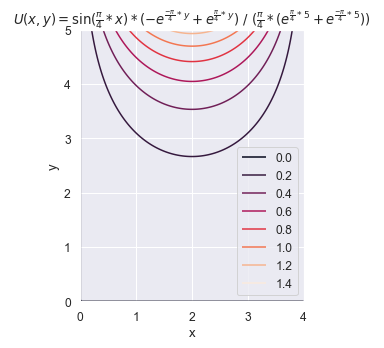
\includegraphics[width=0.8\linewidth]{Dirihle.PNG}

Из этой картины можно увидеть, что решение данной задачи было найдено верно, поскольку на верхней границе прямоугольника $l_{1}\times l_{2}$ происходит изменение потока, а на остальных границах - ничего, что полностью удовлетворяет поставленной задаче.

\pagebreak

\end{document}

